\documentclass[a4paper,12pt]{article}
\usepackage[utf8]{inputenc}
\usepackage{graphicx}
\usepackage{geometry}
\usepackage{amsmath}
\usepackage{hyperref}
\geometry{margin=1in}
\usepackage{float}

\title{Project Report: Weather Station Interface in Java}
\author{Reda El Mansouri \& Dekkan Mohammed}
\date{\today}

\begin{document}
	
	\maketitle	
	
	\tableofcontents
	\newpage
	
	\begin{abstract}
		This report describes the development of a weather station interface using Java and a MySQL database to display real-time weather information. The project also integrates the use of an Arduino microcontroller for climate data collection.
	\end{abstract}
	
	\section{Introduction}
	In this project, we developed a weather station interface that combines modern technologies such as Java, MySQL, and Arduino to provide real-time weather data. This report presents the design details, components used, and tests conducted.
	
	\section{Theme}
	The growing need for accurate climate monitoring motivated this project. The objective was to create a system capable of collecting, storing, and displaying real-time climate data.
	
	\section{Materials and Components Used}
	The main hardware components used in this project are:
	\begin{itemize}
		\item Arduino Microcontroller (model: Arduino Uno)
		\begin{center}
			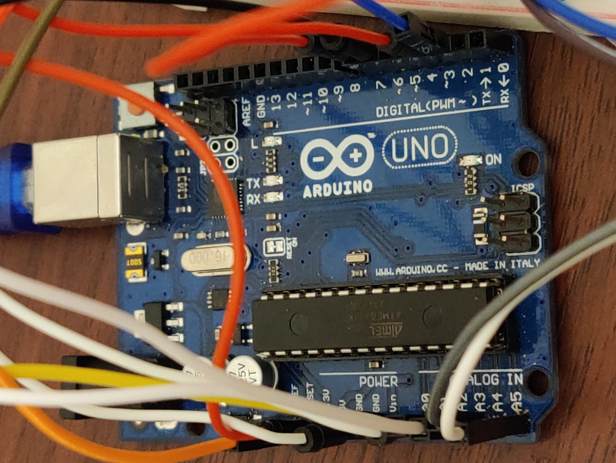
\includegraphics[width=0.8\textwidth]{arduino.png}\\
			\textbf{Figure 1: Arduino Uno Microcontroller}
		\end{center}
		
		\item Humidity and temperature sensors
		\begin{center}
			
\includegraphics[width=0.8\textwidth]{humidity.png}\\
			\textbf{Figure 2: Humidity and Temperature Sensors}
		\end{center}
		
		\item Pressure sensors
		\begin{center}
			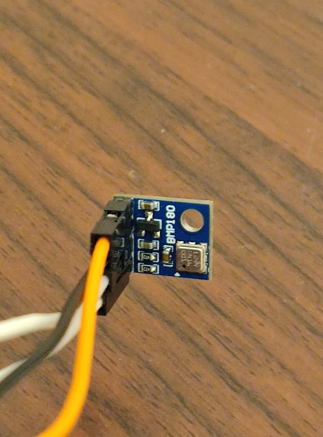
\includegraphics[width=0.8\textwidth]{pressure.png}\\
			\textbf{Figure 3: Pressure Sensor}
		\end{center}
		
		\item Light sensors
		\begin{center}
			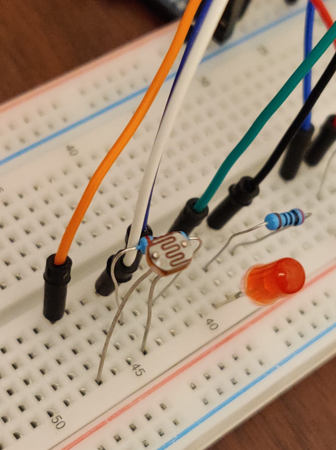
\includegraphics[width=0.8\textwidth]{light.png}\\
			\textbf{Figure 4: Light Sensor}
		\end{center}
		
		\item Rain sensors
		\begin{center}
			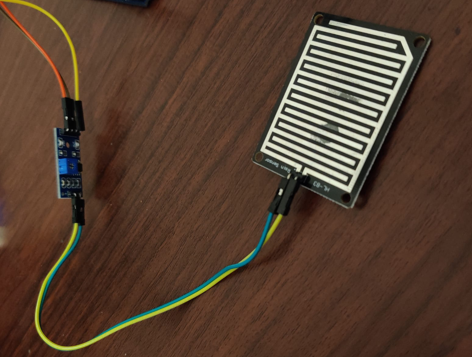
\includegraphics[width=0.8\textwidth]{rain.png}\\
			\textbf{Figure 5: Rain Sensor}
		\end{center}
		
		\item MySQL Database for data storage
		\begin{center}
			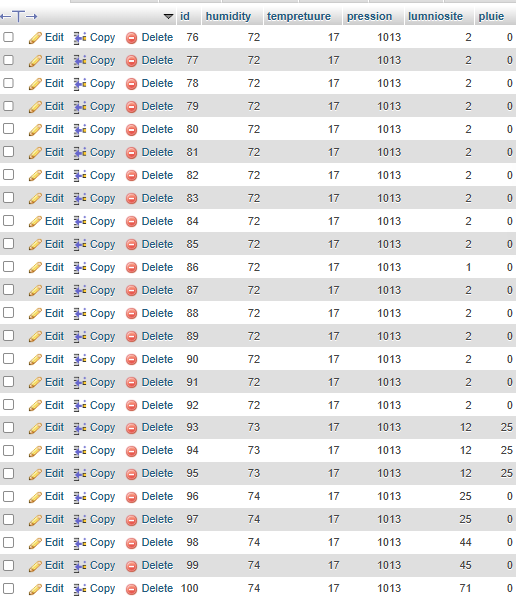
\includegraphics[width=0.8\textwidth]{database.png}\\
			\textbf{Figure 6: MySQL Database}
		\end{center}
	\end{itemize}
	
	\section{Project Architecture}
	The project architecture is divided into three main modules:
	\begin{itemize}
		\item \textbf{Data Collection:} An Arduino microcontroller connected to sensors measures climate parameters such as temperature, humidity, and pressure. The collected data is sent to the host computer via a serial connection.
		\item \textbf{User Interface:} A Java application displays real-time data in the form of graphs and tables. It also includes functionalities to view historical data.
		\item \textbf{Database:} Collected data is stored in a MySQL database for efficient management and future reference.
	\end{itemize}
	
	\section{UML Diagrams}
	This section presents key UML diagrams for the project:
	
	\subsection{Use Case Diagram}
	\begin{center}
		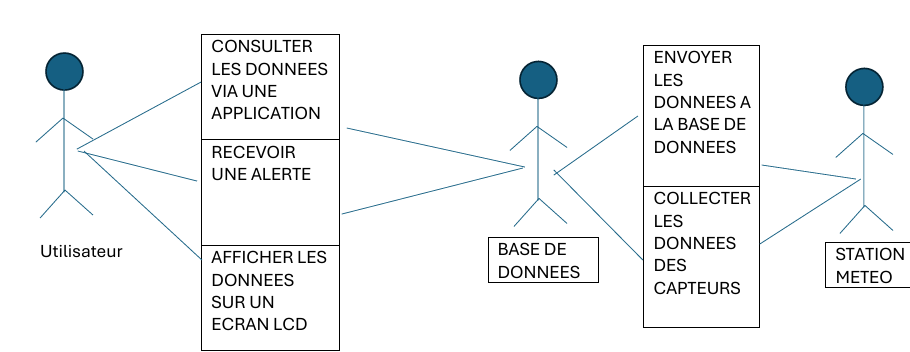
\includegraphics[width=\textwidth]{diagdecas.png}\\
		\textbf{Figure 7: Use Case Diagram}
	\end{center}
	
	\subsection{Class Diagram}
	\begin{center}
		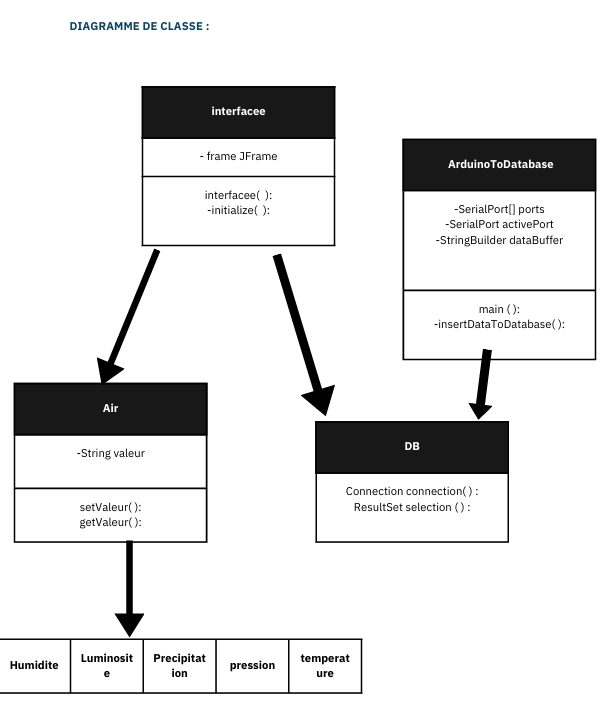
\includegraphics[width=\textwidth]{diagdeclass.png}\\
		\textbf{Figure 8: Class Diagram}
	\end{center}
	
	\subsection{Sequence Diagram}
	\begin{center}
		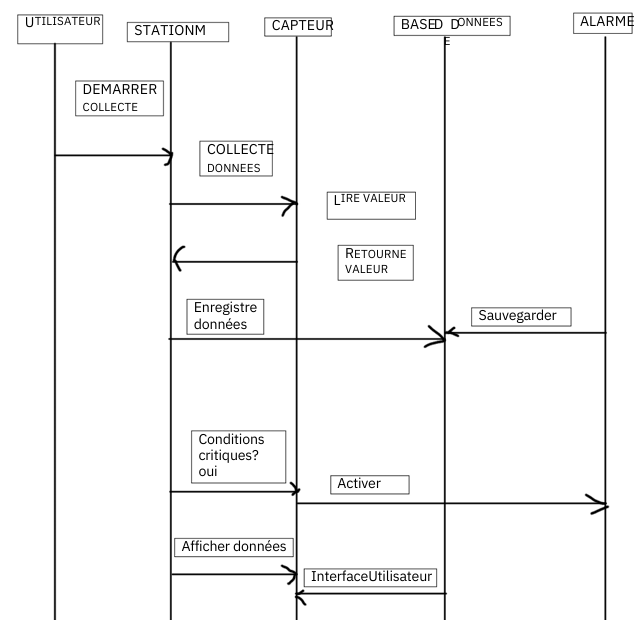
\includegraphics[width=\textwidth]{diagdesueq.png}\\
		\textbf{Figure 9: Sequence Diagram}
	\end{center}
	
	\subsection{Activity Diagram}
	\begin{center}
		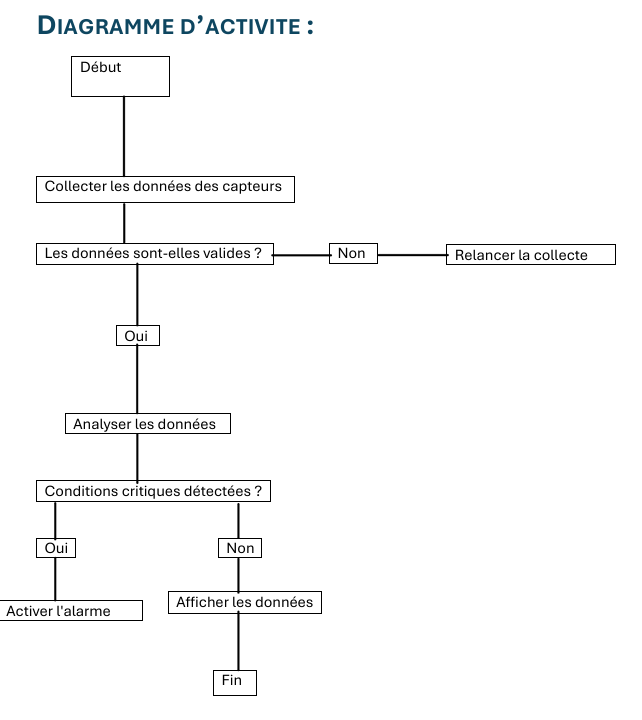
\includegraphics[width=\textwidth]{activity_diagram.png}\\
		\textbf{Figure 10: Activity Diagram}
	\end{center}
	

\section{Unit Test Documentation}
Five unit tests were conducted to validate key application functions. Here is a summary of the tests:

\begin{center}
	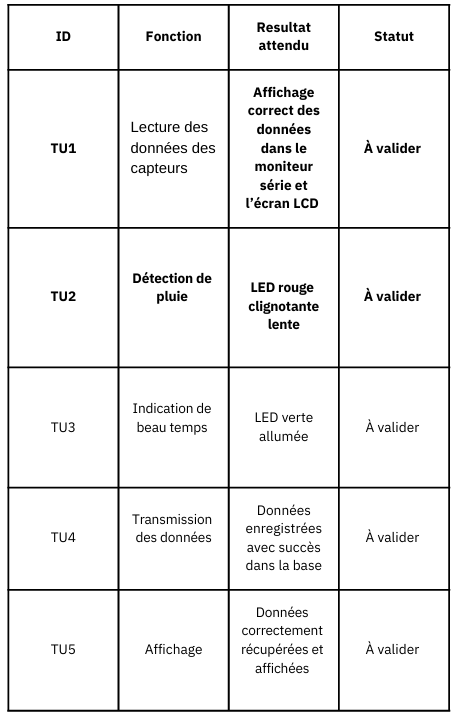
\includegraphics[width=\textwidth]{DTU.png}\\
	\textbf{Figure 11: Unit Test Documentation}
\end{center}

\begin{enumerate}
	\item Reading sensor data: Positive result
	\begin{figure}[H]
		\centering
		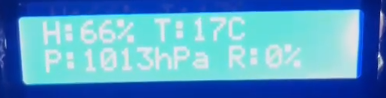
\includegraphics[width=0.8\textwidth]{DTU1.png}
		\caption{Reading sensor data}
		\label{fig:reading_sensor_data}
	\end{figure}
	
	\item Rain detection: Positive result
	\begin{figure}[H]
		\centering
		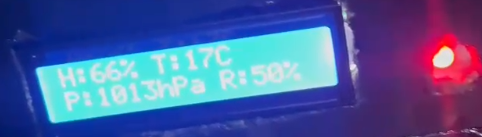
\includegraphics[width=0.8\textwidth]{DTU2.png}
		\caption{Rain detection}
		\label{fig:rain_detection}
	\end{figure}
	
	\item Good weather indication: Positive result
	\begin{figure}[H]
		\centering
		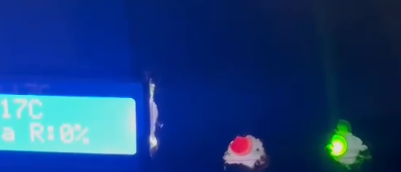
\includegraphics[width=0.8\textwidth]{DTU3.png}
		\caption{Good weather indication}
		\label{fig:good_weather}
	\end{figure}
	
	\item Real-time data update: Positive result
	\begin{figure}[H]
		\centering
		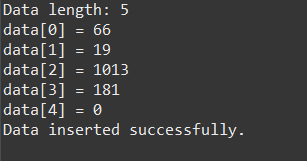
\includegraphics[width=0.8\textwidth]{DTU4(1).png}
		\caption{Real-time data update (Part 1)}
		\label{fig:real_time_update1}
	\end{figure}
	
	\begin{figure}[H]
		\centering
		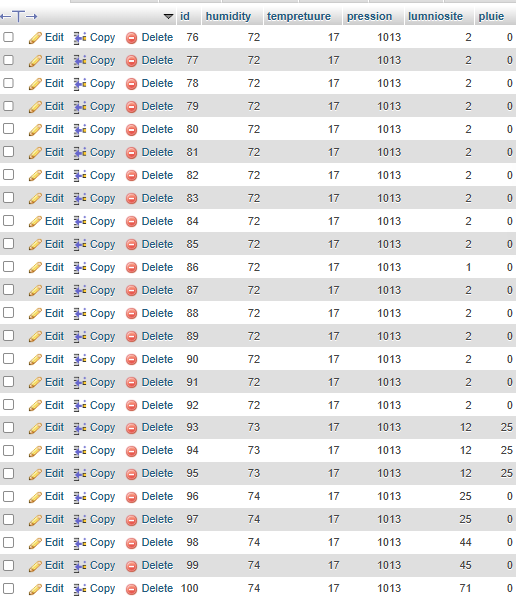
\includegraphics[width=0.8\textwidth]{DTU4(2).png}
		\caption{Real-time data update (Part 2)}
		\label{fig:real_time_update2}
	\end{figure}
	
	\item Display: Positive result
	\begin{figure}[H]
		\centering
		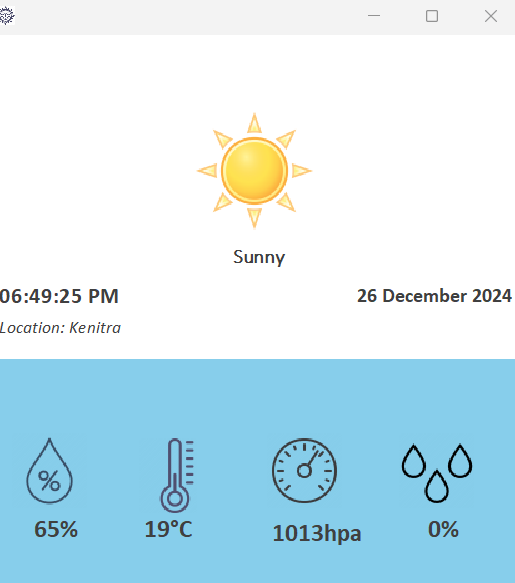
\includegraphics[width=0.8\textwidth]{DTU5.png}
		\caption{Java GUI}
		\label{fig:java_gui}
	\end{figure}
\end{enumerate}


	

	
	\section{Conclusion}
	This project successfully developed a functional and reliable weather station interface using Java for the main application, MySQL for data management, and Arduino for climate data collection. The tests conducted confirm the robustness and efficiency of the system.
	
\end{document}
